\documentclass[1p]{elsarticle_modified}
%\bibliographystyle{elsarticle-num}

%\usepackage[colorlinks]{hyperref}
%\usepackage{abbrmath_seonhwa} %\Abb, \Ascr, \Acal ,\Abf, \Afrak
\usepackage{amsfonts}
\usepackage{amssymb}
\usepackage{amsmath}
\usepackage{amsthm}
\usepackage{scalefnt}
\usepackage{amsbsy}
\usepackage{kotex}
\usepackage{caption}
\usepackage{subfig}
\usepackage{color}
\usepackage{graphicx}
\usepackage{xcolor} %% white, black, red, green, blue, cyan, magenta, yellow
\usepackage{float}
\usepackage{setspace}
\usepackage{hyperref}

\usepackage{tikz}
\usetikzlibrary{arrows}

\usepackage{multirow}
\usepackage{array} % fixed length table
\usepackage{hhline}

%%%%%%%%%%%%%%%%%%%%%
\makeatletter
\renewcommand*\env@matrix[1][\arraystretch]{%
	\edef\arraystretch{#1}%
	\hskip -\arraycolsep
	\let\@ifnextchar\new@ifnextchar
	\array{*\c@MaxMatrixCols c}}
\makeatother %https://tex.stackexchange.com/questions/14071/how-can-i-increase-the-line-spacing-in-a-matrix
%%%%%%%%%%%%%%%

\usepackage[normalem]{ulem}

\newcommand{\msout}[1]{\ifmmode\text{\sout{\ensuremath{#1}}}\else\sout{#1}\fi}
%SOURCE: \msout is \stkout macro in https://tex.stackexchange.com/questions/20609/strikeout-in-math-mode

\newcommand{\cancel}[1]{
	\ifmmode
	{\color{red}\msout{#1}}
	\else
	{\color{red}\sout{#1}}
	\fi
}

\newcommand{\add}[1]{
	{\color{blue}\uwave{#1}}
}

\newcommand{\replace}[2]{
	\ifmmode
	{\color{red}\msout{#1}}{\color{blue}\uwave{#2}}
	\else
	{\color{red}\sout{#1}}{\color{blue}\uwave{#2}}
	\fi
}

\newcommand{\Sol}{\mathcal{S}} %segment
\newcommand{\D}{D} %diagram
\newcommand{\A}{\mathcal{A}} %arc


%%%%%%%%%%%%%%%%%%%%%%%%%%%%%5 test

\def\sl{\operatorname{\textup{SL}}(2,\Cbb)}
\def\psl{\operatorname{\textup{PSL}}(2,\Cbb)}
\def\quan{\mkern 1mu \triangleright \mkern 1mu}

\theoremstyle{definition}
\newtheorem{thm}{Theorem}[section]
\newtheorem{prop}[thm]{Proposition}
\newtheorem{lem}[thm]{Lemma}
\newtheorem{ques}[thm]{Question}
\newtheorem{cor}[thm]{Corollary}
\newtheorem{defn}[thm]{Definition}
\newtheorem{exam}[thm]{Example}
\newtheorem{rmk}[thm]{Remark}
\newtheorem{alg}[thm]{Algorithm}

\newcommand{\I}{\sqrt{-1}}
\begin{document}

%\begin{frontmatter}
%
%\title{Boundary parabolic representations of knots up to 8 crossings}
%
%%% Group authors per affiliation:
%\author{Yunhi Cho} 
%\address{Department of Mathematics, University of Seoul, Seoul, Korea}
%\ead{yhcho@uos.ac.kr}
%
%
%\author{Seonhwa Kim} %\fnref{s_kim}}
%\address{Center for Geometry and Physics, Institute for Basic Science, Pohang, 37673, Korea}
%\ead{ryeona17@ibs.re.kr}
%
%\author{Hyuk Kim}
%\address{Department of Mathematical Sciences, Seoul National University, Seoul 08826, Korea}
%\ead{hyukkim@snu.ac.kr}
%
%\author{Seokbeom Yoon}
%\address{Department of Mathematical Sciences, Seoul National University, Seoul, 08826,  Korea}
%\ead{sbyoon15@snu.ac.kr}
%
%\begin{abstract}
%We find all boundary parabolic representation of knots up to 8 crossings.
%
%\end{abstract}
%\begin{keyword}
%    \MSC[2010] 57M25 
%\end{keyword}
%
%\end{frontmatter}

%\linenumbers
%\tableofcontents
%
\newcommand\colored[1]{\textcolor{white}{\rule[-0.35ex]{0.8em}{1.4ex}}\kern-0.8em\color{red} #1}%
%\newcommand\colored[1]{\textcolor{white}{ #1}\kern-2.17ex	\textcolor{white}{ #1}\kern-1.81ex	\textcolor{white}{ #1}\kern-2.15ex\color{red}#1	}

{\Large $\underline{11n_{172}~(K11n_{172})}$}

\setlength{\tabcolsep}{10pt}
\renewcommand{\arraystretch}{1.6}
\vspace{1cm}\begin{tabular}{m{100pt}>{\centering\arraybackslash}m{274pt}}
\multirow{5}{120pt}{
	\centering
	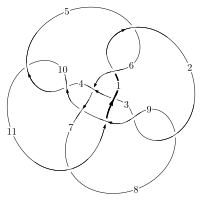
\includegraphics[width=112pt]{../../../GIT/diagram.site/Diagrams/png/788_11n_172.png}\\
\ \ \ A knot diagram\footnotemark}&
\allowdisplaybreaks
\textbf{Linearized knot diagam} \\
\cline{2-2}
 &
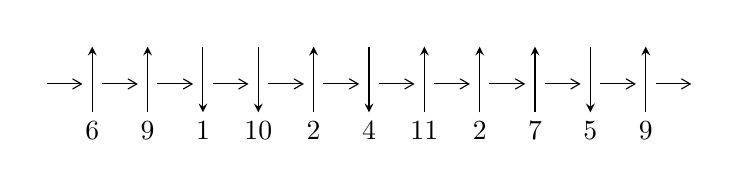
\begin{tikzpicture}[x=20pt, y=17pt]
	% nodes
	\node (C0) at (0, 0) {};
	\node (C1) at (1, 0) {};
	\node (C1U) at (1, +1) {};
	\node (C1D) at (1, -1) {6};

	\node (C2) at (2, 0) {};
	\node (C2U) at (2, +1) {};
	\node (C2D) at (2, -1) {9};

	\node (C3) at (3, 0) {};
	\node (C3U) at (3, +1) {};
	\node (C3D) at (3, -1) {1};

	\node (C4) at (4, 0) {};
	\node (C4U) at (4, +1) {};
	\node (C4D) at (4, -1) {10};

	\node (C5) at (5, 0) {};
	\node (C5U) at (5, +1) {};
	\node (C5D) at (5, -1) {2};

	\node (C6) at (6, 0) {};
	\node (C6U) at (6, +1) {};
	\node (C6D) at (6, -1) {4};

	\node (C7) at (7, 0) {};
	\node (C7U) at (7, +1) {};
	\node (C7D) at (7, -1) {11};

	\node (C8) at (8, 0) {};
	\node (C8U) at (8, +1) {};
	\node (C8D) at (8, -1) {2};

	\node (C9) at (9, 0) {};
	\node (C9U) at (9, +1) {};
	\node (C9D) at (9, -1) {7};

	\node (C10) at (10, 0) {};
	\node (C10U) at (10, +1) {};
	\node (C10D) at (10, -1) {5};

	\node (C11) at (11, 0) {};
	\node (C11U) at (11, +1) {};
	\node (C11D) at (11, -1) {9};
	\node (C12) at (12, 0) {};

	% arrows
	\draw[->,>={angle 60}]
	(C0) edge (C1) (C1) edge (C2) (C2) edge (C3) (C3) edge (C4) (C4) edge (C5) (C5) edge (C6) (C6) edge (C7) (C7) edge (C8) (C8) edge (C9) (C9) edge (C10) (C10) edge (C11) (C11) edge (C12) ;	\draw[->,>=stealth]
	(C1D) edge (C1U) (C2D) edge (C2U) (C3U) edge (C3D) (C4U) edge (C4D) (C5D) edge (C5U) (C6U) edge (C6D) (C7D) edge (C7U) (C8D) edge (C8U) (C9D) edge (C9U) (C10U) edge (C10D) (C11D) edge (C11U) ;
	\end{tikzpicture} \\
\hhline{~~} \\& 
\textbf{Solving Sequence} \\ \cline{2-2} 
 &
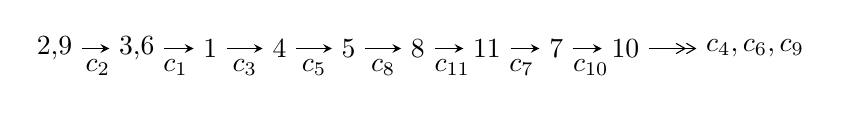
\begin{tikzpicture}[x=25pt, y=7pt]
	% node
	\node (A0) at (-1/8, 0) {2,9};
	\node (A1) at (17/16, 0) {3,6};
	\node (A2) at (17/8, 0) {1};
	\node (A3) at (25/8, 0) {4};
	\node (A4) at (33/8, 0) {5};
	\node (A5) at (41/8, 0) {8};
	\node (A6) at (49/8, 0) {11};
	\node (A7) at (57/8, 0) {7};
	\node (A8) at (65/8, 0) {10};
	\node (C1) at (1/2, -1) {$c_{2}$};
	\node (C2) at (13/8, -1) {$c_{1}$};
	\node (C3) at (21/8, -1) {$c_{3}$};
	\node (C4) at (29/8, -1) {$c_{5}$};
	\node (C5) at (37/8, -1) {$c_{8}$};
	\node (C6) at (45/8, -1) {$c_{11}$};
	\node (C7) at (53/8, -1) {$c_{7}$};
	\node (C8) at (61/8, -1) {$c_{10}$};
	\node (A9) at (10, 0) {$c_{4},c_{6},c_{9}$};

	% edge
	\draw[->,>=stealth]	
	(A0) edge (A1) (A1) edge (A2) (A2) edge (A3) (A3) edge (A4) (A4) edge (A5) (A5) edge (A6) (A6) edge (A7) (A7) edge (A8) ;
	\draw[->>,>={angle 60}]	
	(A8) edge (A9);
\end{tikzpicture} \\ 

\end{tabular} \\

\footnotetext{
The image of knot diagram is generated by the software ``\textbf{Draw programme}" developed by Andrew Bartholomew(\url{http://www.layer8.co.uk/maths/draw/index.htm\#Running-draw}), where we modified some parts for our purpose(\url{https://github.com/CATsTAILs/LinksPainter}).
}\phantom \\ \newline 
\centering \textbf{Ideals for irreducible components\footnotemark of $X_{\text{par}}$} 
 
\begin{align*}
I^u_{1}&=\langle 
2.80403\times10^{129} u^{39}+1.00269\times10^{129} u^{38}+\cdots+1.55952\times10^{133} b-4.83307\times10^{132},\\
\phantom{I^u_{1}}&\phantom{= \langle  }3.18557\times10^{131} u^{39}-1.42090\times10^{132} u^{38}+\cdots+6.95548\times10^{135} a+3.12217\times10^{135},\\
\phantom{I^u_{1}}&\phantom{= \langle  }u^{40}- u^{39}+\cdots+492 u-892\rangle \\
I^u_{2}&=\langle 
-3007418546 u^{15}+933342897 u^{14}+\cdots+9161883482 b+4813387670,\\
\phantom{I^u_{2}}&\phantom{= \langle  }-1873381418 u^{15}-2988794220 u^{14}+\cdots+9161883482 a-21851752726,\\
\phantom{I^u_{2}}&\phantom{= \langle  }u^{16}+5 u^{14}-5 u^{13}- u^{11}-24 u^{10}+16 u^9+4 u^8-16 u^7+20 u^6-4 u^5-17 u^4+4 u^3+10 u^2-4\rangle \\
\\
\end{align*}
\raggedright * 2 irreducible components of $\dim_{\mathbb{C}}=0$, with total 56 representations.\\
\footnotetext{All coefficients of polynomials are rational numbers. But the coefficients are sometimes approximated in decimal forms when there is not enough margin.}
\newpage
\renewcommand{\arraystretch}{1}
\centering \section*{I. $I^u_{1}= \langle 2.80\times10^{129} u^{39}+1.00\times10^{129} u^{38}+\cdots+1.56\times10^{133} b-4.83\times10^{132},\;3.19\times10^{131} u^{39}-1.42\times10^{132} u^{38}+\cdots+6.96\times10^{135} a+3.12\times10^{135},\;u^{40}- u^{39}+\cdots+492 u-892 \rangle$}
\flushleft \textbf{(i) Arc colorings}\\
\begin{tabular}{m{7pt} m{180pt} m{7pt} m{180pt} }
\flushright $a_{2}=$&$\begin{pmatrix}1\\0\end{pmatrix}$ \\
\flushright $a_{9}=$&$\begin{pmatrix}0\\u\end{pmatrix}$ \\
\flushright $a_{3}=$&$\begin{pmatrix}1\\- u^2\end{pmatrix}$ \\
\flushright $a_{6}=$&$\begin{pmatrix}-0.0000457994 u^{39}+0.000204285 u^{38}+\cdots+0.0708298 u-0.448879\\-0.000179801 u^{39}-0.0000642943 u^{38}+\cdots+1.95559 u+0.309907\end{pmatrix}$ \\
\flushright $a_{1}=$&$\begin{pmatrix}0.0000420568 u^{39}-0.000112360 u^{38}+\cdots-2.24245 u+0.0906996\\-0.000731650 u^{39}+0.000562011 u^{38}+\cdots+0.278566 u-0.727739\end{pmatrix}$ \\
\flushright $a_{4}=$&$\begin{pmatrix}-0.000151445 u^{39}-0.0000710102 u^{38}+\cdots+2.55187 u+2.12193\\0.000373065 u^{39}-0.000239614 u^{38}+\cdots-0.711429 u+0.439973\end{pmatrix}$ \\
\flushright $a_{5}=$&$\begin{pmatrix}0.000134001 u^{39}+0.000268580 u^{38}+\cdots-1.88476 u-0.758785\\-0.000179801 u^{39}-0.0000642943 u^{38}+\cdots+1.95559 u+0.309907\end{pmatrix}$ \\
\flushright $a_{8}=$&$\begin{pmatrix}- u\\u\end{pmatrix}$ \\
\flushright $a_{11}=$&$\begin{pmatrix}0.0000420568 u^{39}-0.000112360 u^{38}+\cdots-2.24245 u+0.0906996\\-0.000736091 u^{39}+0.000525007 u^{38}+\cdots+0.350670 u-0.790450\end{pmatrix}$ \\
\flushright $a_{7}=$&$\begin{pmatrix}0.000166450 u^{39}-0.000130525 u^{38}+\cdots-1.45638 u+1.06015\\0.000220629 u^{39}-0.0000136383 u^{38}+\cdots-0.303665 u-0.108440\end{pmatrix}$ \\
\flushright $a_{10}=$&$\begin{pmatrix}-0.000515912 u^{39}+0.000203912 u^{38}+\cdots-0.148443 u-0.735075\\-0.000308939 u^{39}+0.000237175 u^{38}+\cdots-0.241184 u-0.390016\end{pmatrix}$\\ \flushright $a_{10}=$&$\begin{pmatrix}-0.000515912 u^{39}+0.000203912 u^{38}+\cdots-0.148443 u-0.735075\\-0.000308939 u^{39}+0.000237175 u^{38}+\cdots-0.241184 u-0.390016\end{pmatrix}$\\&\end{tabular}
\flushleft \textbf{(ii) Obstruction class $= -1$}\\~\\
\flushleft \textbf{(iii) Cusp Shapes $= -0.000707464 u^{39}-0.00139771 u^{38}+\cdots-3.97400 u-0.836131$}\\~\\
\newpage\renewcommand{\arraystretch}{1}
\flushleft \textbf{(iv) u-Polynomials at the component}\newline \\
\begin{tabular}{m{50pt}|m{274pt}}
Crossings & \hspace{64pt}u-Polynomials at each crossing \\
\hline $$\begin{aligned}c_{1},c_{5}\end{aligned}$$&$\begin{aligned}
&u^{40}-2 u^{39}+\cdots+14 u-1
\end{aligned}$\\
\hline $$\begin{aligned}c_{2},c_{8}\end{aligned}$$&$\begin{aligned}
&u^{40}- u^{39}+\cdots+492 u-892
\end{aligned}$\\
\hline $$\begin{aligned}c_{3}\end{aligned}$$&$\begin{aligned}
&u^{40}-5 u^{39}+\cdots-248 u+88
\end{aligned}$\\
\hline $$\begin{aligned}c_{4},c_{10}\end{aligned}$$&$\begin{aligned}
&u^{40}- u^{39}+\cdots-12 u+4
\end{aligned}$\\
\hline $$\begin{aligned}c_{6}\end{aligned}$$&$\begin{aligned}
&u^{40}-5 u^{39}+\cdots+457 u+29
\end{aligned}$\\
\hline $$\begin{aligned}c_{7}\end{aligned}$$&$\begin{aligned}
&u^{40}-3 u^{39}+\cdots-26575 u+7349
\end{aligned}$\\
\hline $$\begin{aligned}c_{9}\end{aligned}$$&$\begin{aligned}
&u^{40}+5 u^{39}+\cdots+96 u+11
\end{aligned}$\\
\hline $$\begin{aligned}c_{11}\end{aligned}$$&$\begin{aligned}
&u^{40}+u^{39}+\cdots-1168 u-424
\end{aligned}$\\
\hline
\end{tabular}\\~\\
\newpage\renewcommand{\arraystretch}{1}
\flushleft \textbf{(v) Riley Polynomials at the component}\newline \\
\begin{tabular}{m{50pt}|m{274pt}}
Crossings & \hspace{64pt}Riley Polynomials at each crossing \\
\hline $$\begin{aligned}c_{1},c_{5}\end{aligned}$$&$\begin{aligned}
&y^{40}+38 y^{39}+\cdots-78 y+1
\end{aligned}$\\
\hline $$\begin{aligned}c_{2},c_{8}\end{aligned}$$&$\begin{aligned}
&y^{40}+63 y^{39}+\cdots+6026912 y+795664
\end{aligned}$\\
\hline $$\begin{aligned}c_{3}\end{aligned}$$&$\begin{aligned}
&y^{40}-59 y^{39}+\cdots-199840 y+7744
\end{aligned}$\\
\hline $$\begin{aligned}c_{4},c_{10}\end{aligned}$$&$\begin{aligned}
&y^{40}-35 y^{39}+\cdots+1888 y+16
\end{aligned}$\\
\hline $$\begin{aligned}c_{6}\end{aligned}$$&$\begin{aligned}
&y^{40}-15 y^{39}+\cdots-262383 y+841
\end{aligned}$\\
\hline $$\begin{aligned}c_{7}\end{aligned}$$&$\begin{aligned}
&y^{40}+47 y^{39}+\cdots+923130863 y+54007801
\end{aligned}$\\
\hline $$\begin{aligned}c_{9}\end{aligned}$$&$\begin{aligned}
&y^{40}+7 y^{39}+\cdots-218 y+121
\end{aligned}$\\
\hline $$\begin{aligned}c_{11}\end{aligned}$$&$\begin{aligned}
&y^{40}+57 y^{39}+\cdots+1150944 y+179776
\end{aligned}$\\
\hline
\end{tabular}\\~\\
\newpage\flushleft \textbf{(vi) Complex Volumes and Cusp Shapes}
$$\begin{array}{c|c|c}  
\text{Solutions to }I^u_{1}& \I (\text{vol} + \sqrt{-1}CS) & \text{Cusp shape}\\
 \hline 
\begin{aligned}
u &= -0.972209 + 0.363644 I \\
a &= -0.691473 - 0.726212 I \\
b &= \phantom{-}0.246524 - 1.044100 I\end{aligned}
 & -1.63884 - 2.52981 I & -3.46896 + 4.78238 I \\ \hline\begin{aligned}
u &= -0.972209 - 0.363644 I \\
a &= -0.691473 + 0.726212 I \\
b &= \phantom{-}0.246524 + 1.044100 I\end{aligned}
 & -1.63884 + 2.52981 I & -3.46896 - 4.78238 I \\ \hline\begin{aligned}
u &= -0.777438 + 0.253101 I \\
a &= -0.28608 - 2.07418 I \\
b &= \phantom{-}0.0965200 - 0.0759702 I\end{aligned}
 & -0.55843 - 5.04023 I & \phantom{-}8.92316 + 6.11668 I \\ \hline\begin{aligned}
u &= -0.777438 - 0.253101 I \\
a &= -0.28608 + 2.07418 I \\
b &= \phantom{-}0.0965200 + 0.0759702 I\end{aligned}
 & -0.55843 + 5.04023 I & \phantom{-}8.92316 - 6.11668 I \\ \hline\begin{aligned}
u &= -1.028590 + 0.641044 I \\
a &= \phantom{-}0.812402 + 0.180660 I \\
b &= -0.05196 + 1.65626 I\end{aligned}
 & -6.89381 + 4.31374 I & -3.00921 - 2.52408 I \\ \hline\begin{aligned}
u &= -1.028590 - 0.641044 I \\
a &= \phantom{-}0.812402 - 0.180660 I \\
b &= -0.05196 - 1.65626 I\end{aligned}
 & -6.89381 - 4.31374 I & -3.00921 + 2.52408 I \\ \hline\begin{aligned}
u &= \phantom{-}1.28769\phantom{ +0.000000I} \\
a &= -1.23762\phantom{ +0.000000I} \\
b &= \phantom{-}1.21545\phantom{ +0.000000I}\end{aligned}
 & \phantom{-}2.31916\phantom{ +0.000000I} & \phantom{-}3.45590\phantom{ +0.000000I} \\ \hline\begin{aligned}
u &= -0.004586 + 0.662077 I \\
a &= -0.110517 - 1.374950 I \\
b &= -0.440412 - 1.198770 I\end{aligned}
 & -6.21063 + 2.44288 I & -1.57019 - 3.53786 I \\ \hline\begin{aligned}
u &= -0.004586 - 0.662077 I \\
a &= -0.110517 + 1.374950 I \\
b &= -0.440412 + 1.198770 I\end{aligned}
 & -6.21063 - 2.44288 I & -1.57019 + 3.53786 I \\ \hline\begin{aligned}
u &= \phantom{-}0.606580 + 0.241726 I \\
a &= -0.989022 - 0.886345 I \\
b &= \phantom{-}0.197863 + 0.060558 I\end{aligned}
 & \phantom{-}1.31470 + 0.60771 I & \phantom{-}8.49421 - 3.04989 I\\
 \hline 
 \end{array}$$\newpage$$\begin{array}{c|c|c}  
\text{Solutions to }I^u_{1}& \I (\text{vol} + \sqrt{-1}CS) & \text{Cusp shape}\\
 \hline 
\begin{aligned}
u &= \phantom{-}0.606580 - 0.241726 I \\
a &= -0.989022 + 0.886345 I \\
b &= \phantom{-}0.197863 - 0.060558 I\end{aligned}
 & \phantom{-}1.31470 - 0.60771 I & \phantom{-}8.49421 + 3.04989 I \\ \hline\begin{aligned}
u &= \phantom{-}0.584454 + 0.231728 I \\
a &= -0.083035 + 1.313620 I \\
b &= -0.458127 + 1.196180 I\end{aligned}
 & -5.71740 - 6.20191 I & -6.05433 + 5.08780 I \\ \hline\begin{aligned}
u &= \phantom{-}0.584454 - 0.231728 I \\
a &= -0.083035 - 1.313620 I \\
b &= -0.458127 - 1.196180 I\end{aligned}
 & -5.71740 + 6.20191 I & -6.05433 - 5.08780 I \\ \hline\begin{aligned}
u &= -0.607336\phantom{ +0.000000I} \\
a &= \phantom{-}2.89129\phantom{ +0.000000I} \\
b &= -1.09842\phantom{ +0.000000I}\end{aligned}
 & \phantom{-}3.09539\phantom{ +0.000000I} & -9.16160\phantom{ +0.000000I} \\ \hline\begin{aligned}
u &= \phantom{-}0.13576 + 1.42105 I \\
a &= -0.158909 - 0.108207 I \\
b &= -0.742397 - 0.144685 I\end{aligned}
 & -4.59373 + 2.98825 I & \phantom{-}4.81250 - 3.01552 I \\ \hline\begin{aligned}
u &= \phantom{-}0.13576 - 1.42105 I \\
a &= -0.158909 + 0.108207 I \\
b &= -0.742397 + 0.144685 I\end{aligned}
 & -4.59373 - 2.98825 I & \phantom{-}4.81250 + 3.01552 I \\ \hline\begin{aligned}
u &= -0.292078 + 0.391717 I \\
a &= -0.559269 + 0.026373 I \\
b &= -0.768195 + 0.090718 I\end{aligned}
 & -2.47058 + 1.70720 I & \phantom{-}0.230221 - 0.591796 I \\ \hline\begin{aligned}
u &= -0.292078 - 0.391717 I \\
a &= -0.559269 - 0.026373 I \\
b &= -0.768195 - 0.090718 I\end{aligned}
 & -2.47058 - 1.70720 I & \phantom{-}0.230221 + 0.591796 I \\ \hline\begin{aligned}
u &= \phantom{-}0.011693 + 0.471366 I \\
a &= -0.639263 - 0.198812 I \\
b &= \phantom{-}0.381500 + 0.672173 I\end{aligned}
 & \phantom{-}0.03644 + 1.50292 I & \phantom{-}1.25089 - 6.14683 I \\ \hline\begin{aligned}
u &= \phantom{-}0.011693 - 0.471366 I \\
a &= -0.639263 + 0.198812 I \\
b &= \phantom{-}0.381500 - 0.672173 I\end{aligned}
 & \phantom{-}0.03644 - 1.50292 I & \phantom{-}1.25089 + 6.14683 I\\
 \hline 
 \end{array}$$\newpage$$\begin{array}{c|c|c}  
\text{Solutions to }I^u_{1}& \I (\text{vol} + \sqrt{-1}CS) & \text{Cusp shape}\\
 \hline 
\begin{aligned}
u &= \phantom{-}0.281701 + 0.359944 I \\
a &= -2.19829 - 0.09585 I \\
b &= \phantom{-}0.325667 + 1.141170 I\end{aligned}
 & -1.21242 + 1.07873 I & -3.63948 + 1.17826 I \\ \hline\begin{aligned}
u &= \phantom{-}0.281701 - 0.359944 I \\
a &= -2.19829 + 0.09585 I \\
b &= \phantom{-}0.325667 - 1.141170 I\end{aligned}
 & -1.21242 - 1.07873 I & -3.63948 - 1.17826 I \\ \hline\begin{aligned}
u &= -0.11719 + 1.62482 I \\
a &= \phantom{-}0.403686 - 0.292336 I \\
b &= -0.345255 - 0.125454 I\end{aligned}
 & -8.09181 - 0.67197 I & \phantom{-0.000000 } 0 \\ \hline\begin{aligned}
u &= -0.11719 - 1.62482 I \\
a &= \phantom{-}0.403686 + 0.292336 I \\
b &= -0.345255 + 0.125454 I\end{aligned}
 & -8.09181 + 0.67197 I & \phantom{-0.000000 } 0 \\ \hline\begin{aligned}
u &= \phantom{-}1.60181 + 1.05960 I \\
a &= \phantom{-}0.323648 - 0.513185 I \\
b &= \phantom{-}0.10749 - 1.61398 I\end{aligned}
 & -6.22320 + 3.43752 I & \phantom{-0.000000 } 0 \\ \hline\begin{aligned}
u &= \phantom{-}1.60181 - 1.05960 I \\
a &= \phantom{-}0.323648 + 0.513185 I \\
b &= \phantom{-}0.10749 + 1.61398 I\end{aligned}
 & -6.22320 - 3.43752 I & \phantom{-0.000000 } 0 \\ \hline\begin{aligned}
u &= -0.48768 + 1.87046 I \\
a &= \phantom{-}0.445879 + 1.224510 I \\
b &= -0.14644 + 1.58425 I\end{aligned}
 & -14.3940 - 1.3454 I & \phantom{-0.000000 } 0 \\ \hline\begin{aligned}
u &= -0.48768 - 1.87046 I \\
a &= \phantom{-}0.445879 - 1.224510 I \\
b &= -0.14644 - 1.58425 I\end{aligned}
 & -14.3940 + 1.3454 I & \phantom{-0.000000 } 0 \\ \hline\begin{aligned}
u &= -0.11349 + 1.97784 I \\
a &= \phantom{-}0.128360 + 1.333720 I \\
b &= -0.27705 + 1.55024 I\end{aligned}
 & -10.55230 - 6.76566 I & \phantom{-0.000000 } 0 \\ \hline\begin{aligned}
u &= -0.11349 - 1.97784 I \\
a &= \phantom{-}0.128360 - 1.333720 I \\
b &= -0.27705 - 1.55024 I\end{aligned}
 & -10.55230 + 6.76566 I & \phantom{-0.000000 } 0\\
 \hline 
 \end{array}$$\newpage$$\begin{array}{c|c|c}  
\text{Solutions to }I^u_{1}& \I (\text{vol} + \sqrt{-1}CS) & \text{Cusp shape}\\
 \hline 
\begin{aligned}
u &= -0.00542 + 2.12395 I \\
a &= \phantom{-}0.124816 - 1.215410 I \\
b &= -0.28024 - 1.51688 I\end{aligned}
 & -9.55118 + 0.96633 I & \phantom{-0.000000 } 0 \\ \hline\begin{aligned}
u &= -0.00542 - 2.12395 I \\
a &= \phantom{-}0.124816 + 1.215410 I \\
b &= -0.28024 + 1.51688 I\end{aligned}
 & -9.55118 - 0.96633 I & \phantom{-0.000000 } 0 \\ \hline\begin{aligned}
u &= \phantom{-}0.21330 + 2.22331 I \\
a &= -0.0303329 + 0.0193746 I \\
b &= \phantom{-}1.75447 - 0.27463 I\end{aligned}
 & -10.09040 - 5.18311 I & \phantom{-0.000000 } 0 \\ \hline\begin{aligned}
u &= \phantom{-}0.21330 - 2.22331 I \\
a &= -0.0303329 - 0.0193746 I \\
b &= \phantom{-}1.75447 + 0.27463 I\end{aligned}
 & -10.09040 + 5.18311 I & \phantom{-0.000000 } 0 \\ \hline\begin{aligned}
u &= -0.79762 + 2.19173 I \\
a &= -0.440868 - 0.873034 I \\
b &= \phantom{-}0.84317 - 1.82666 I\end{aligned}
 & -14.8294 - 4.4956 I & \phantom{-0.000000 } 0 \\ \hline\begin{aligned}
u &= -0.79762 - 2.19173 I \\
a &= -0.440868 + 0.873034 I \\
b &= \phantom{-}0.84317 + 1.82666 I\end{aligned}
 & -14.8294 + 4.4956 I & \phantom{-0.000000 } 0 \\ \hline\begin{aligned}
u &= \phantom{-}0.56414 + 2.26378 I \\
a &= -0.363789 + 1.003570 I \\
b &= \phantom{-}0.63008 + 1.69717 I\end{aligned}
 & -16.3560 + 13.3915 I & \phantom{-0.000000 } 0 \\ \hline\begin{aligned}
u &= \phantom{-}0.56414 - 2.26378 I \\
a &= -0.363789 - 1.003570 I \\
b &= \phantom{-}0.63008 - 1.69717 I\end{aligned}
 & -16.3560 - 13.3915 I & \phantom{-0.000000 } 0 \\ \hline\begin{aligned}
u &= \phantom{-}0.75669 + 2.48566 I \\
a &= \phantom{-}0.256526 - 1.062360 I \\
b &= -0.13173 - 1.46303 I\end{aligned}
 & -12.97920 + 2.42998 I & \phantom{-0.000000 } 0 \\ \hline\begin{aligned}
u &= \phantom{-}0.75669 - 2.48566 I \\
a &= \phantom{-}0.256526 + 1.062360 I \\
b &= -0.13173 + 1.46303 I\end{aligned}
 & -12.97920 - 2.42998 I & \phantom{-0.000000 } 0\\
 \hline 
 \end{array}$$\newpage\newpage\renewcommand{\arraystretch}{1}
\centering \section*{II. $I^u_{2}= \langle -3.01\times10^{9} u^{15}+9.33\times10^{8} u^{14}+\cdots+9.16\times10^{9} b+4.81\times10^{9},\;-1.87\times10^{9} u^{15}-2.99\times10^{9} u^{14}+\cdots+9.16\times10^{9} a-2.19\times10^{10},\;u^{16}+5 u^{14}+\cdots+10 u^2-4 \rangle$}
\flushleft \textbf{(i) Arc colorings}\\
\begin{tabular}{m{7pt} m{180pt} m{7pt} m{180pt} }
\flushright $a_{2}=$&$\begin{pmatrix}1\\0\end{pmatrix}$ \\
\flushright $a_{9}=$&$\begin{pmatrix}0\\u\end{pmatrix}$ \\
\flushright $a_{3}=$&$\begin{pmatrix}1\\- u^2\end{pmatrix}$ \\
\flushright $a_{6}=$&$\begin{pmatrix}0.204476 u^{15}+0.326221 u^{14}+\cdots-0.0881222 u+2.38507\\0.328253 u^{15}-0.101872 u^{14}+\cdots+1.42300 u-0.525371\end{pmatrix}$ \\
\flushright $a_{1}=$&$\begin{pmatrix}0.197482 u^{15}-0.179148 u^{14}+\cdots+1.09215 u-1.18979\\-0.196147 u^{15}+0.172594 u^{14}+\cdots-1.16409 u+0.366552\end{pmatrix}$ \\
\flushright $a_{4}=$&$\begin{pmatrix}-0.0632878 u^{15}-0.0676739 u^{14}+\cdots-0.398063 u+1.03749\\-0.00954759 u^{15}+0.0961985 u^{14}+\cdots-0.151211 u+0.663053\end{pmatrix}$ \\
\flushright $a_{5}=$&$\begin{pmatrix}-0.123778 u^{15}+0.428093 u^{14}+\cdots-1.51112 u+2.91044\\0.328253 u^{15}-0.101872 u^{14}+\cdots+1.42300 u-0.525371\end{pmatrix}$ \\
\flushright $a_{8}=$&$\begin{pmatrix}- u\\u\end{pmatrix}$ \\
\flushright $a_{11}=$&$\begin{pmatrix}0.197482 u^{15}-0.179148 u^{14}+\cdots+1.09215 u-1.18979\\-0.0923248 u^{15}+0.0842185 u^{14}+\cdots-0.374160 u-0.350040\end{pmatrix}$ \\
\flushright $a_{7}=$&$\begin{pmatrix}-0.0660443 u^{15}+0.133020 u^{14}+\cdots-2.18472 u+1.03736\\0.0529067 u^{15}+0.140450 u^{14}+\cdots+0.570148 u+0.302746\end{pmatrix}$ \\
\flushright $a_{10}=$&$\begin{pmatrix}-0.0419856 u^{15}-0.418545 u^{14}+\cdots+1.04104 u-2.75923\\-0.120621 u^{15}-0.0702787 u^{14}+\cdots-0.632997 u-0.128181\end{pmatrix}$\\ \flushright $a_{10}=$&$\begin{pmatrix}-0.0419856 u^{15}-0.418545 u^{14}+\cdots+1.04104 u-2.75923\\-0.120621 u^{15}-0.0702787 u^{14}+\cdots-0.632997 u-0.128181\end{pmatrix}$\\&\end{tabular}
\flushleft \textbf{(ii) Obstruction class $= 1$}\\~\\
\flushleft \textbf{(iii) Cusp Shapes $= -\frac{7739992772}{4580941741} u^{15}+\frac{9173770896}{4580941741} u^{14}+\cdots-\frac{57525934822}{4580941741} u+\frac{47024714230}{4580941741}$}\\~\\
\newpage\renewcommand{\arraystretch}{1}
\flushleft \textbf{(iv) u-Polynomials at the component}\newline \\
\begin{tabular}{m{50pt}|m{274pt}}
Crossings & \hspace{64pt}u-Polynomials at each crossing \\
\hline $$\begin{aligned}c_{1}\end{aligned}$$&$\begin{aligned}
&u^{16}- u^{15}+\cdots-2 u-1
\end{aligned}$\\
\hline $$\begin{aligned}c_{2}\end{aligned}$$&$\begin{aligned}
&u^{16}+5 u^{14}+\cdots+10 u^2-4
\end{aligned}$\\
\hline $$\begin{aligned}c_{3}\end{aligned}$$&$\begin{aligned}
&u^{16}+8 u^{15}+\cdots+12 u+8
\end{aligned}$\\
\hline $$\begin{aligned}c_{4}\end{aligned}$$&$\begin{aligned}
&u^{16}-6 u^{14}+\cdots-14 u^2+4
\end{aligned}$\\
\hline $$\begin{aligned}c_{5}\end{aligned}$$&$\begin{aligned}
&u^{16}+u^{15}+\cdots+2 u-1
\end{aligned}$\\
\hline $$\begin{aligned}c_{6}\end{aligned}$$&$\begin{aligned}
&u^{16}+2 u^{15}+\cdots+11 u+1
\end{aligned}$\\
\hline $$\begin{aligned}c_{7}\end{aligned}$$&$\begin{aligned}
&u^{16}-2 u^{15}+\cdots+13 u+1
\end{aligned}$\\
\hline $$\begin{aligned}c_{8}\end{aligned}$$&$\begin{aligned}
&u^{16}+5 u^{14}+\cdots+10 u^2-4
\end{aligned}$\\
\hline $$\begin{aligned}c_{9}\end{aligned}$$&$\begin{aligned}
&u^{16}-6 u^{15}+\cdots-2 u+1
\end{aligned}$\\
\hline $$\begin{aligned}c_{10}\end{aligned}$$&$\begin{aligned}
&u^{16}-6 u^{14}+\cdots-14 u^2+4
\end{aligned}$\\
\hline $$\begin{aligned}c_{11}\end{aligned}$$&$\begin{aligned}
&u^{16}+4 u^{14}+\cdots+4 u^2-1
\end{aligned}$\\
\hline
\end{tabular}\\~\\
\newpage\renewcommand{\arraystretch}{1}
\flushleft \textbf{(v) Riley Polynomials at the component}\newline \\
\begin{tabular}{m{50pt}|m{274pt}}
Crossings & \hspace{64pt}Riley Polynomials at each crossing \\
\hline $$\begin{aligned}c_{1},c_{5}\end{aligned}$$&$\begin{aligned}
&y^{16}+9 y^{15}+\cdots+10 y+1
\end{aligned}$\\
\hline $$\begin{aligned}c_{2},c_{8}\end{aligned}$$&$\begin{aligned}
&y^{16}+10 y^{15}+\cdots-80 y+16
\end{aligned}$\\
\hline $$\begin{aligned}c_{3}\end{aligned}$$&$\begin{aligned}
&y^{16}-20 y^{15}+\cdots-1168 y+64
\end{aligned}$\\
\hline $$\begin{aligned}c_{4},c_{10}\end{aligned}$$&$\begin{aligned}
&y^{16}-12 y^{15}+\cdots-112 y+16
\end{aligned}$\\
\hline $$\begin{aligned}c_{6}\end{aligned}$$&$\begin{aligned}
&y^{16}+4 y^{14}+\cdots-91 y+1
\end{aligned}$\\
\hline $$\begin{aligned}c_{7}\end{aligned}$$&$\begin{aligned}
&y^{16}+10 y^{15}+\cdots-69 y+1
\end{aligned}$\\
\hline $$\begin{aligned}c_{9}\end{aligned}$$&$\begin{aligned}
&y^{16}-2 y^{15}+\cdots-2 y+1
\end{aligned}$\\
\hline $$\begin{aligned}c_{11}\end{aligned}$$&$\begin{aligned}
&y^{16}+8 y^{15}+\cdots-8 y+1
\end{aligned}$\\
\hline
\end{tabular}\\~\\
\newpage\flushleft \textbf{(vi) Complex Volumes and Cusp Shapes}
$$\begin{array}{c|c|c}  
\text{Solutions to }I^u_{2}& \I (\text{vol} + \sqrt{-1}CS) & \text{Cusp shape}\\
 \hline 
\begin{aligned}
u &= -1.044910 + 0.084383 I \\
a &= \phantom{-}0.057226 + 0.245893 I \\
b &= \phantom{-}0.361947 + 1.340670 I\end{aligned}
 & -4.61886 + 6.15067 I & \phantom{-}1.67402 - 4.95826 I \\ \hline\begin{aligned}
u &= -1.044910 - 0.084383 I \\
a &= \phantom{-}0.057226 - 0.245893 I \\
b &= \phantom{-}0.361947 - 1.340670 I\end{aligned}
 & -4.61886 - 6.15067 I & \phantom{-}1.67402 + 4.95826 I \\ \hline\begin{aligned}
u &= \phantom{-}0.203156 + 1.098810 I \\
a &= -0.741658 - 0.024758 I \\
b &= -0.379929 - 0.431781 I\end{aligned}
 & -5.56667 + 2.95635 I & -4.74772 - 2.75237 I \\ \hline\begin{aligned}
u &= \phantom{-}0.203156 - 1.098810 I \\
a &= -0.741658 + 0.024758 I \\
b &= -0.379929 + 0.431781 I\end{aligned}
 & -5.56667 - 2.95635 I & -4.74772 + 2.75237 I \\ \hline\begin{aligned}
u &= \phantom{-}0.701325 + 0.516464 I \\
a &= \phantom{-}1.021890 - 0.280960 I \\
b &= -0.299377 - 1.065240 I\end{aligned}
 & -0.62726 + 1.86405 I & \phantom{-}2.38240 - 3.76150 I \\ \hline\begin{aligned}
u &= \phantom{-}0.701325 - 0.516464 I \\
a &= \phantom{-}1.021890 + 0.280960 I \\
b &= -0.299377 + 1.065240 I\end{aligned}
 & -0.62726 - 1.86405 I & \phantom{-}2.38240 + 3.76150 I \\ \hline\begin{aligned}
u &= -0.813758\phantom{ +0.000000I} \\
a &= \phantom{-}2.21481\phantom{ +0.000000I} \\
b &= -1.08888\phantom{ +0.000000I}\end{aligned}
 & \phantom{-}3.38602\phantom{ +0.000000I} & \phantom{-}19.6050\phantom{ +0.000000I} \\ \hline\begin{aligned}
u &= \phantom{-}0.752983 + 0.179131 I \\
a &= \phantom{-}0.79516 - 2.54506 I \\
b &= -0.050757 - 0.668728 I\end{aligned}
 & -1.13425 + 5.09162 I & -5.21325 - 6.81011 I \\ \hline\begin{aligned}
u &= \phantom{-}0.752983 - 0.179131 I \\
a &= \phantom{-}0.79516 + 2.54506 I \\
b &= -0.050757 + 0.668728 I\end{aligned}
 & -1.13425 - 5.09162 I & -5.21325 + 6.81011 I \\ \hline\begin{aligned}
u &= -0.474047 + 0.462486 I \\
a &= \phantom{-}1.29761 - 1.51241 I \\
b &= -0.190166 - 0.829536 I\end{aligned}
 & \phantom{-}0.363930 + 0.209601 I & \phantom{-}0.372974 + 0.607008 I\\
 \hline 
 \end{array}$$\newpage$$\begin{array}{c|c|c}  
\text{Solutions to }I^u_{2}& \I (\text{vol} + \sqrt{-1}CS) & \text{Cusp shape}\\
 \hline 
\begin{aligned}
u &= -0.474047 - 0.462486 I \\
a &= \phantom{-}1.29761 + 1.51241 I \\
b &= -0.190166 + 0.829536 I\end{aligned}
 & \phantom{-}0.363930 - 0.209601 I & \phantom{-}0.372974 - 0.607008 I \\ \hline\begin{aligned}
u &= \phantom{-}1.43010\phantom{ +0.000000I} \\
a &= -1.12981\phantom{ +0.000000I} \\
b &= \phantom{-}1.62094\phantom{ +0.000000I}\end{aligned}
 & \phantom{-}1.43155\phantom{ +0.000000I} & -5.25650\phantom{ +0.000000I} \\ \hline\begin{aligned}
u &= \phantom{-}0.13607 + 1.51148 I \\
a &= -0.173098 - 0.201972 I \\
b &= \phantom{-}0.597072 - 0.748618 I\end{aligned}
 & -8.25349 - 1.91163 I & -5.00806 + 3.84199 I \\ \hline\begin{aligned}
u &= \phantom{-}0.13607 - 1.51148 I \\
a &= -0.173098 + 0.201972 I \\
b &= \phantom{-}0.597072 + 0.748618 I\end{aligned}
 & -8.25349 + 1.91163 I & -5.00806 - 3.84199 I \\ \hline\begin{aligned}
u &= -0.58274 + 2.26201 I \\
a &= -0.299629 - 1.085740 I \\
b &= \phantom{-}0.19518 - 1.54614 I\end{aligned}
 & -12.18100 - 1.94801 I & -0.634861 - 0.077298 I \\ \hline\begin{aligned}
u &= -0.58274 - 2.26201 I \\
a &= -0.299629 + 1.085740 I \\
b &= \phantom{-}0.19518 + 1.54614 I\end{aligned}
 & -12.18100 + 1.94801 I & -0.634861 + 0.077298 I\\
 \hline 
 \end{array}$$\newpage
\newpage\renewcommand{\arraystretch}{1}
\centering \section*{ III. u-Polynomials}
\begin{tabular}{m{50pt}|m{274pt}}
Crossings & \hspace{64pt}u-Polynomials at each crossing \\
\hline $$\begin{aligned}c_{1}\end{aligned}$$&$\begin{aligned}
&(u^{16}- u^{15}+\cdots-2 u-1)(u^{40}-2 u^{39}+\cdots+14 u-1)
\end{aligned}$\\
\hline $$\begin{aligned}c_{2}\end{aligned}$$&$\begin{aligned}
&(u^{16}+5 u^{14}+\cdots+10 u^2-4)(u^{40}- u^{39}+\cdots+492 u-892)
\end{aligned}$\\
\hline $$\begin{aligned}c_{3}\end{aligned}$$&$\begin{aligned}
&(u^{16}+8 u^{15}+\cdots+12 u+8)(u^{40}-5 u^{39}+\cdots-248 u+88)
\end{aligned}$\\
\hline $$\begin{aligned}c_{4}\end{aligned}$$&$\begin{aligned}
&(u^{16}-6 u^{14}+\cdots-14 u^2+4)(u^{40}- u^{39}+\cdots-12 u+4)
\end{aligned}$\\
\hline $$\begin{aligned}c_{5}\end{aligned}$$&$\begin{aligned}
&(u^{16}+u^{15}+\cdots+2 u-1)(u^{40}-2 u^{39}+\cdots+14 u-1)
\end{aligned}$\\
\hline $$\begin{aligned}c_{6}\end{aligned}$$&$\begin{aligned}
&(u^{16}+2 u^{15}+\cdots+11 u+1)(u^{40}-5 u^{39}+\cdots+457 u+29)
\end{aligned}$\\
\hline $$\begin{aligned}c_{7}\end{aligned}$$&$\begin{aligned}
&(u^{16}-2 u^{15}+\cdots+13 u+1)(u^{40}-3 u^{39}+\cdots-26575 u+7349)
\end{aligned}$\\
\hline $$\begin{aligned}c_{8}\end{aligned}$$&$\begin{aligned}
&(u^{16}+5 u^{14}+\cdots+10 u^2-4)(u^{40}- u^{39}+\cdots+492 u-892)
\end{aligned}$\\
\hline $$\begin{aligned}c_{9}\end{aligned}$$&$\begin{aligned}
&(u^{16}-6 u^{15}+\cdots-2 u+1)(u^{40}+5 u^{39}+\cdots+96 u+11)
\end{aligned}$\\
\hline $$\begin{aligned}c_{10}\end{aligned}$$&$\begin{aligned}
&(u^{16}-6 u^{14}+\cdots-14 u^2+4)(u^{40}- u^{39}+\cdots-12 u+4)
\end{aligned}$\\
\hline $$\begin{aligned}c_{11}\end{aligned}$$&$\begin{aligned}
&(u^{16}+4 u^{14}+\cdots+4 u^2-1)(u^{40}+u^{39}+\cdots-1168 u-424)
\end{aligned}$\\
\hline
\end{tabular}\newpage\renewcommand{\arraystretch}{1}
\centering \section*{ IV. Riley Polynomials}
\begin{tabular}{m{50pt}|m{274pt}}
Crossings & \hspace{64pt}Riley Polynomials at each crossing \\
\hline $$\begin{aligned}c_{1},c_{5}\end{aligned}$$&$\begin{aligned}
&(y^{16}+9 y^{15}+\cdots+10 y+1)(y^{40}+38 y^{39}+\cdots-78 y+1)
\end{aligned}$\\
\hline $$\begin{aligned}c_{2},c_{8}\end{aligned}$$&$\begin{aligned}
&(y^{16}+10 y^{15}+\cdots-80 y+16)\\
&\cdot(y^{40}+63 y^{39}+\cdots+6026912 y+795664)
\end{aligned}$\\
\hline $$\begin{aligned}c_{3}\end{aligned}$$&$\begin{aligned}
&(y^{16}-20 y^{15}+\cdots-1168 y+64)\\
&\cdot(y^{40}-59 y^{39}+\cdots-199840 y+7744)
\end{aligned}$\\
\hline $$\begin{aligned}c_{4},c_{10}\end{aligned}$$&$\begin{aligned}
&(y^{16}-12 y^{15}+\cdots-112 y+16)(y^{40}-35 y^{39}+\cdots+1888 y+16)
\end{aligned}$\\
\hline $$\begin{aligned}c_{6}\end{aligned}$$&$\begin{aligned}
&(y^{16}+4 y^{14}+\cdots-91 y+1)(y^{40}-15 y^{39}+\cdots-262383 y+841)
\end{aligned}$\\
\hline $$\begin{aligned}c_{7}\end{aligned}$$&$\begin{aligned}
&(y^{16}+10 y^{15}+\cdots-69 y+1)\\
&\cdot(y^{40}+47 y^{39}+\cdots+923130863 y+54007801)
\end{aligned}$\\
\hline $$\begin{aligned}c_{9}\end{aligned}$$&$\begin{aligned}
&(y^{16}-2 y^{15}+\cdots-2 y+1)(y^{40}+7 y^{39}+\cdots-218 y+121)
\end{aligned}$\\
\hline $$\begin{aligned}c_{11}\end{aligned}$$&$\begin{aligned}
&(y^{16}+8 y^{15}+\cdots-8 y+1)(y^{40}+57 y^{39}+\cdots+1150944 y+179776)
\end{aligned}$\\
\hline
\end{tabular}
\vskip 2pc
\end{document}